\chapter{Results and Interpretation}\label{sec:results}

Figures~\ref{fig:3}~and~\ref{fig:4} show the $m_{\ell^+\ell^-\gamma}$ distributions of the data events in each category.
The expected SM $\PH\to\PZ\gamma$ distributions, scaled by a factor of 10, are also shown.
Figure~\ref{fig:SignalBackground} shows the signal-plus-background fit to the data and the corresponding distribution after background subtraction for the sum of all categories. 
Each category is weighted by the factor $S/(S+B)$, where $S$ is the expected signal yield  
and $B$ is the background yield in the narrowest mass interval containing 95\% of the signal distribution.

\begin{figure}
  \centering
  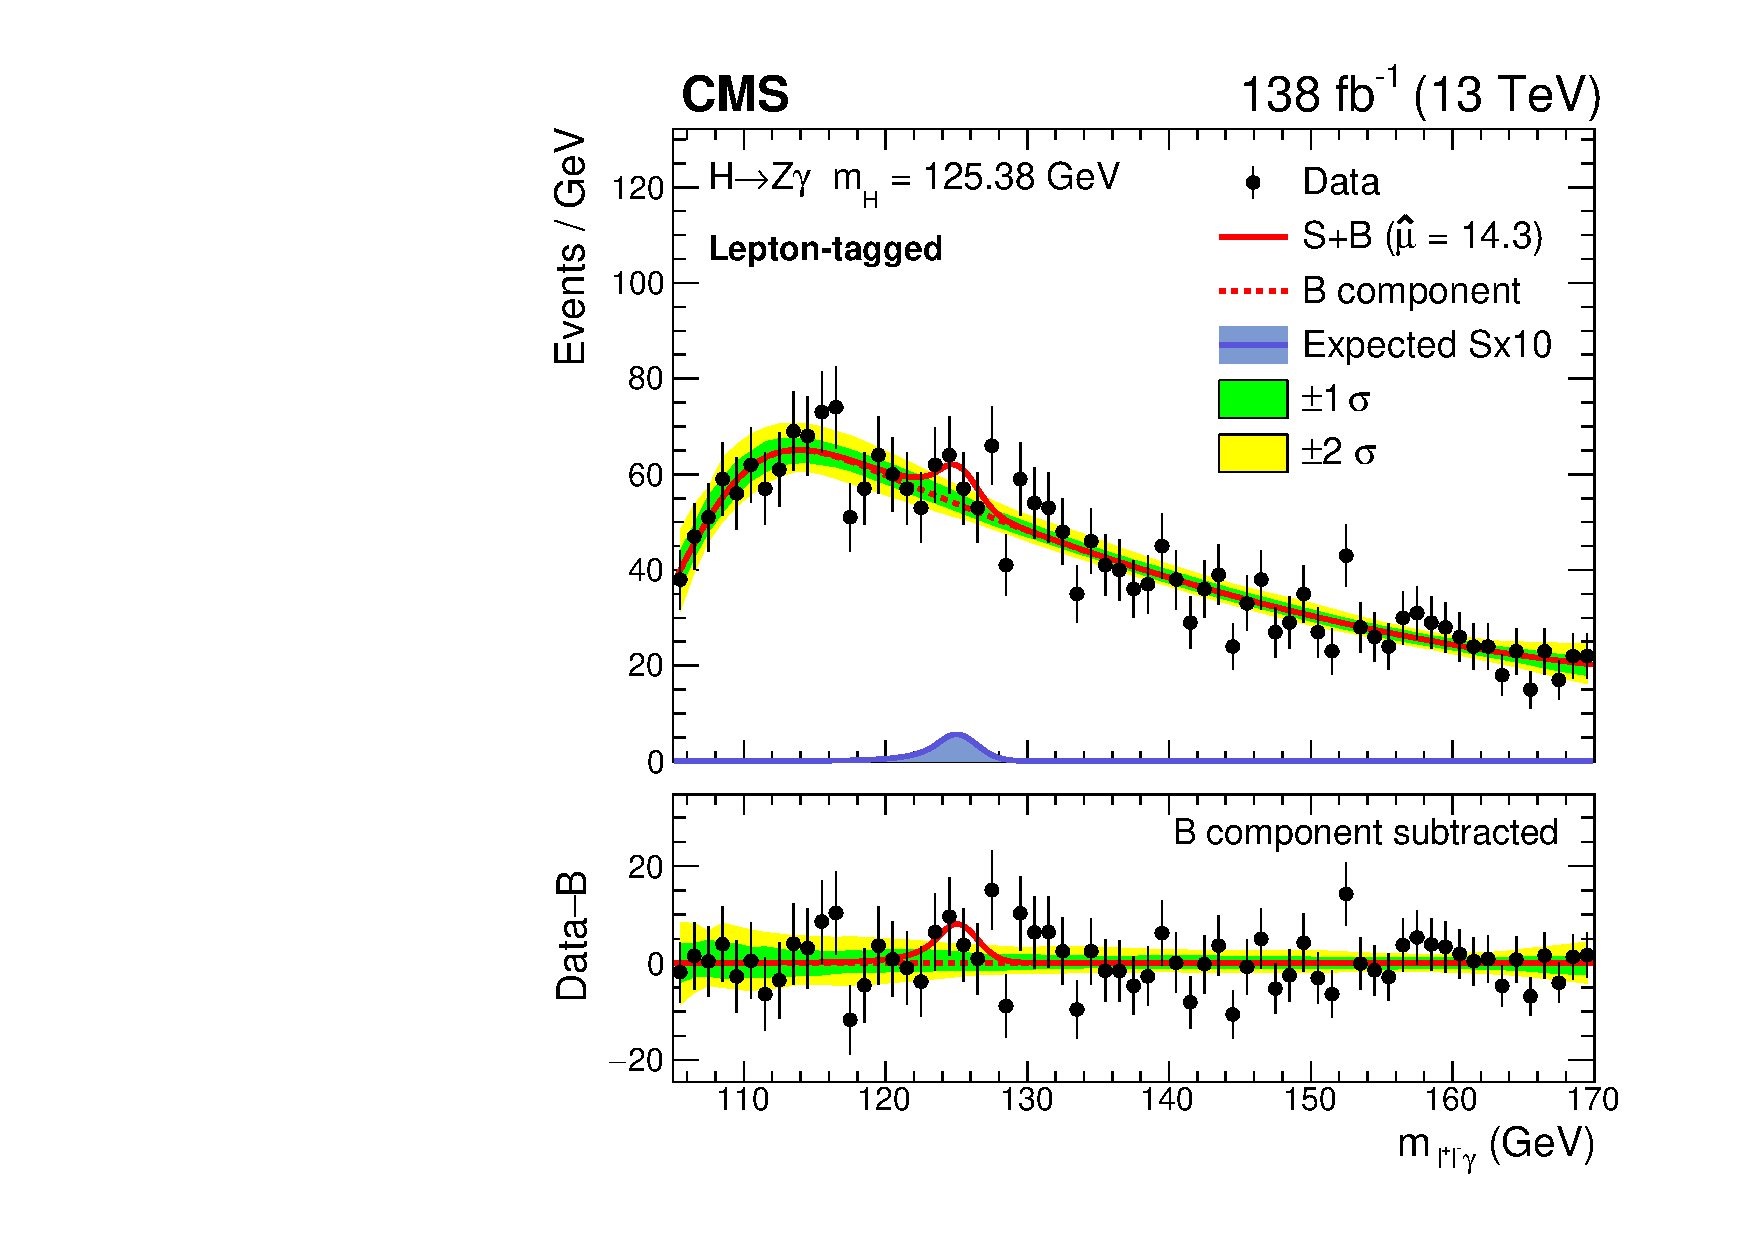
\includegraphics[width=0.45\textwidth]{fig/results/Figure_008.pdf}
  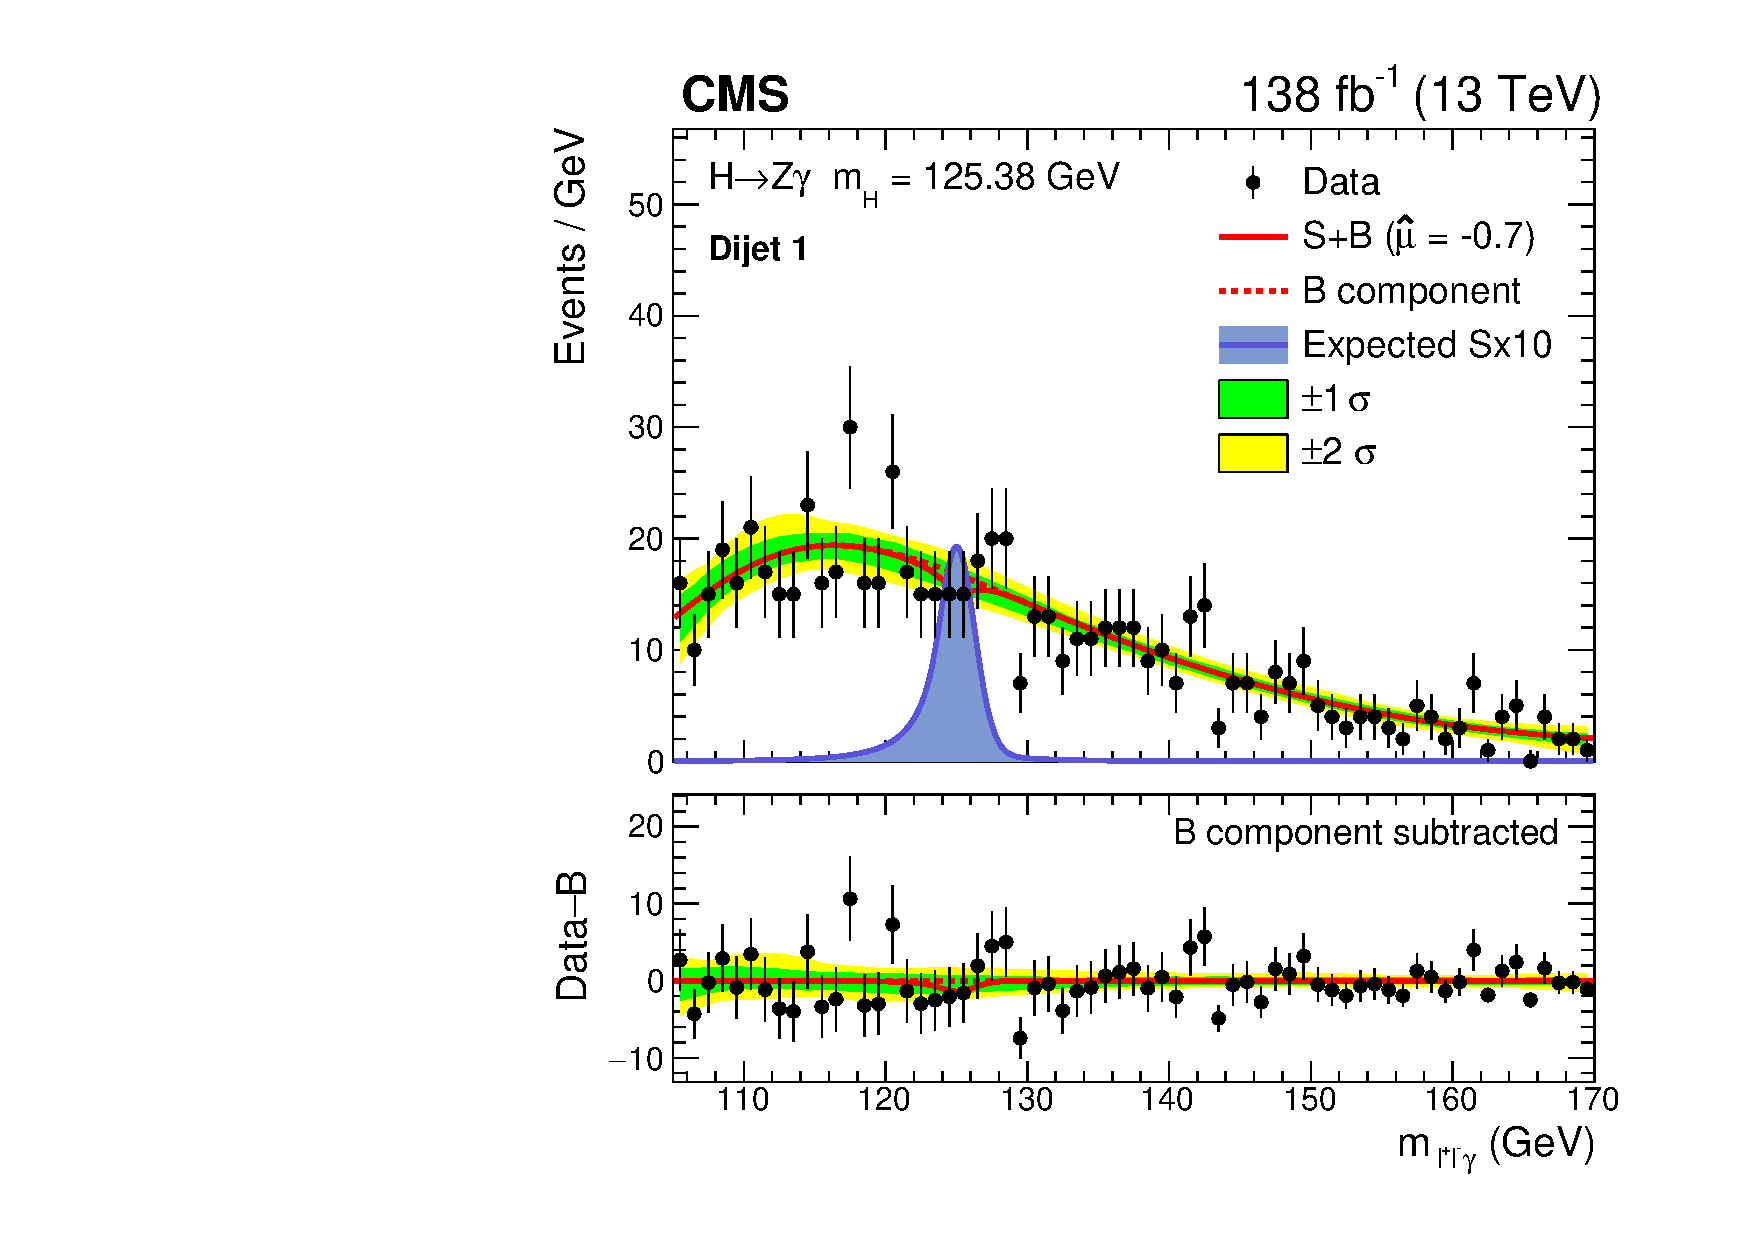
\includegraphics[width=0.45\textwidth]{fig/results/Figure_004-a.pdf}\\
  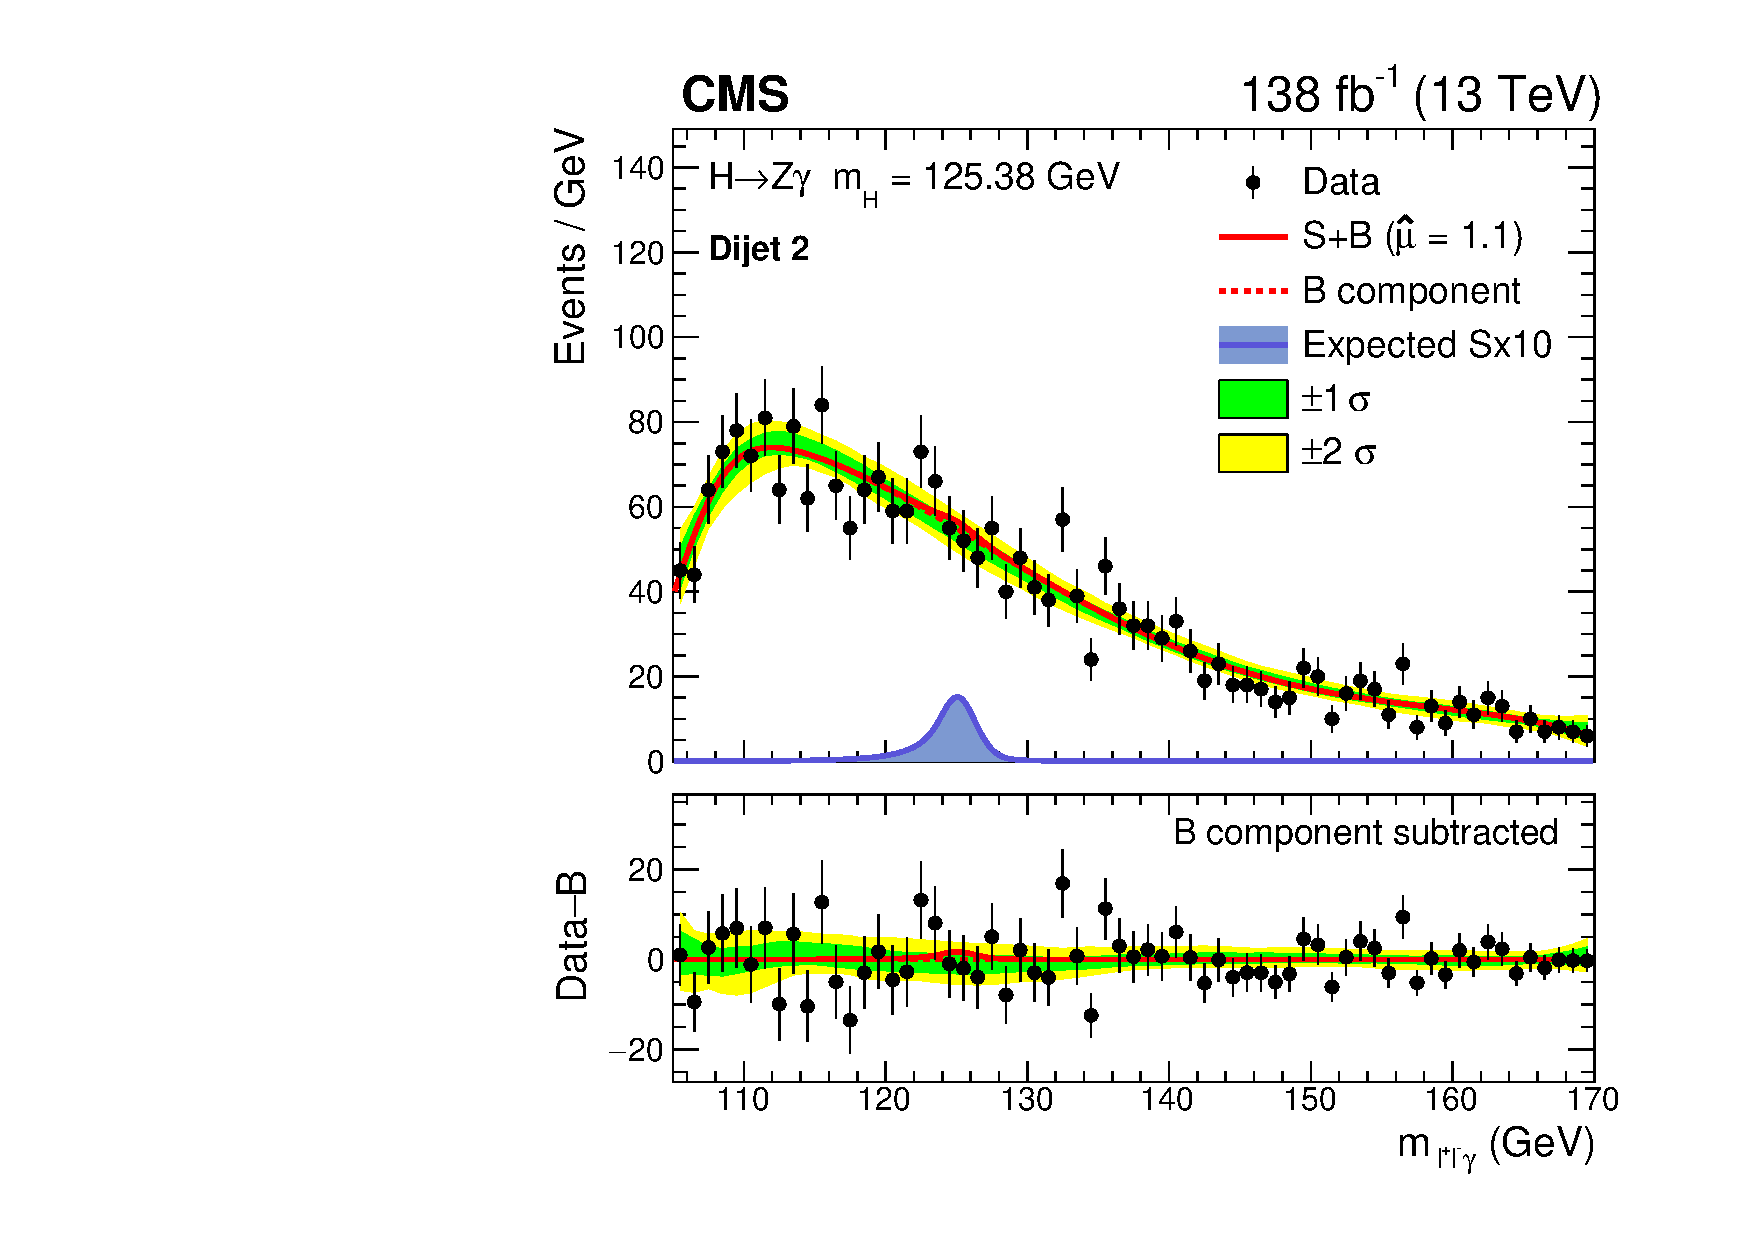
\includegraphics[width=0.45\textwidth]{fig/results/Figure_004-b.pdf}
  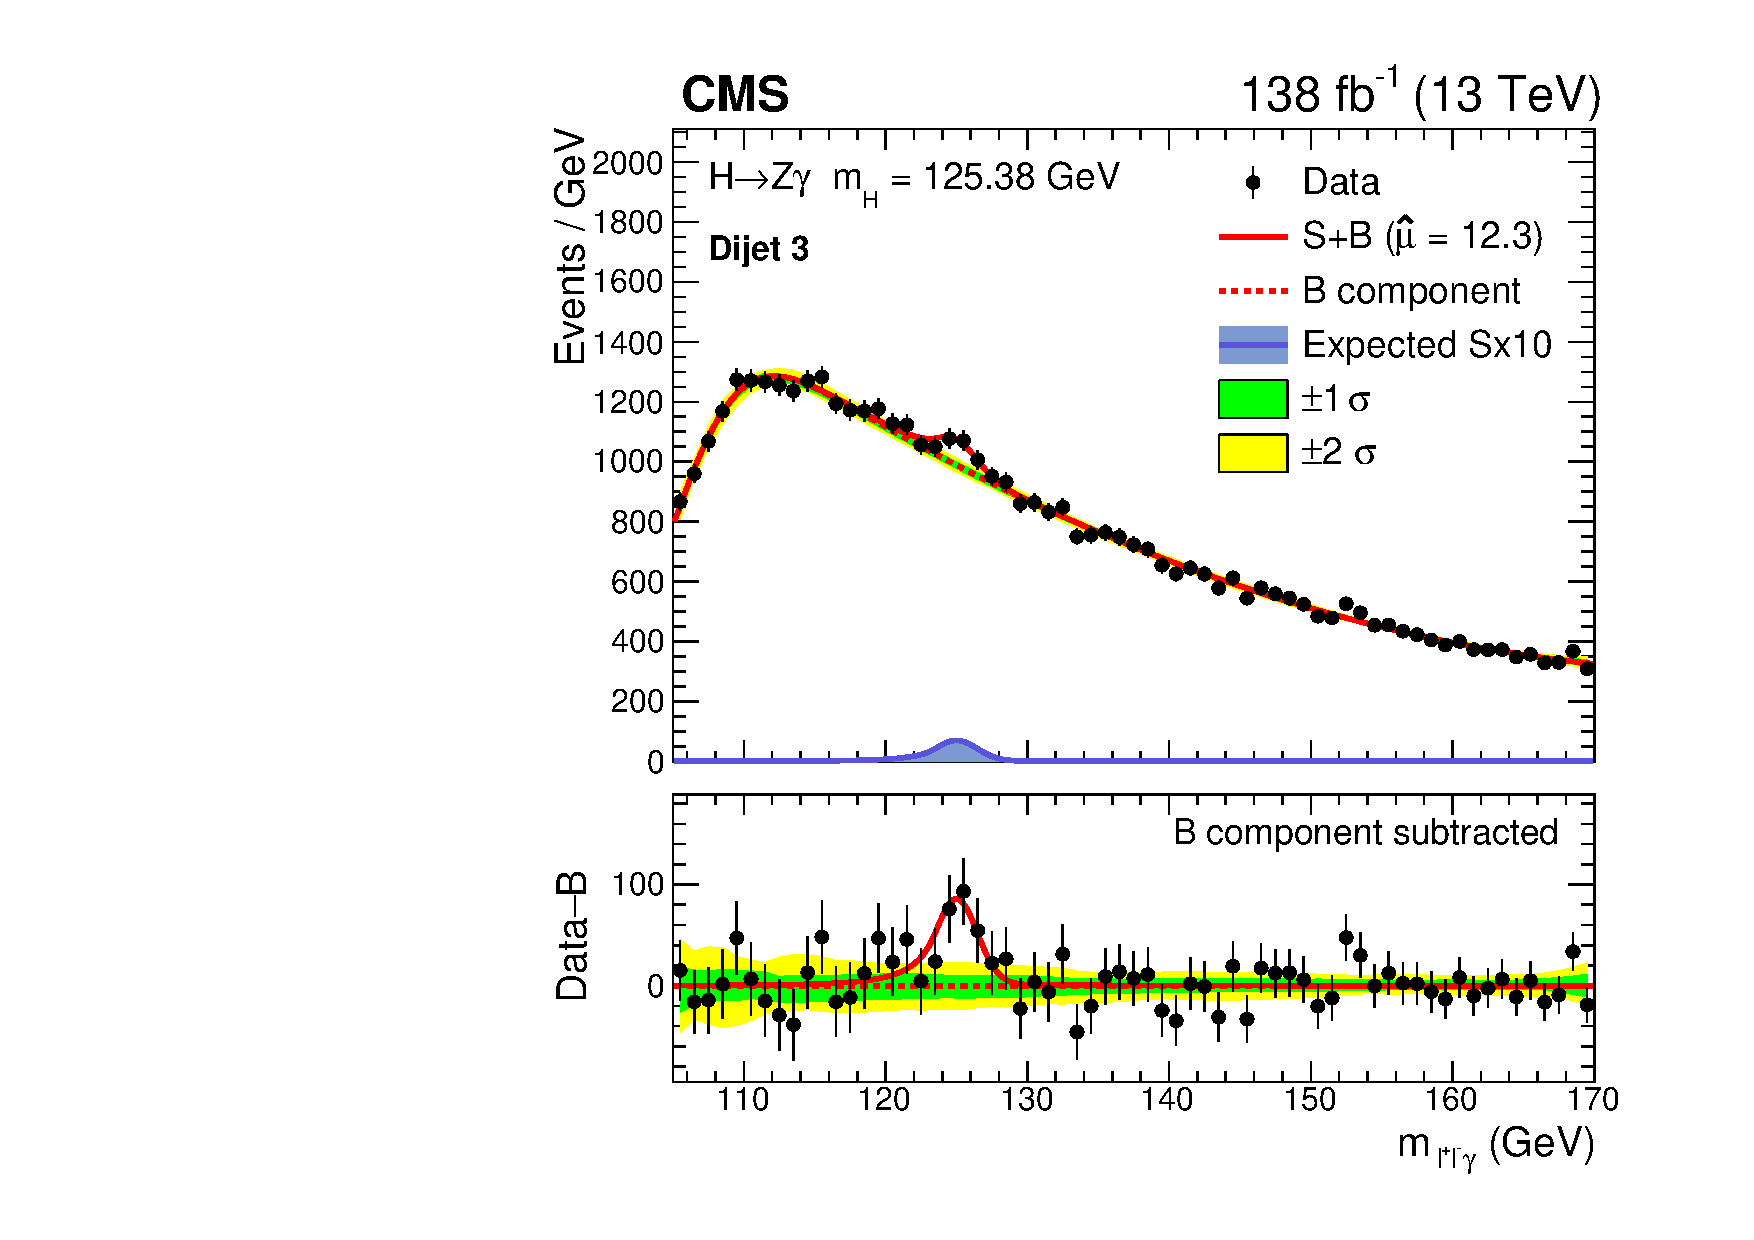
\includegraphics[width=0.45\textwidth]{fig/results/Figure_004-c.pdf}\\
   \caption{Fits to the $m_{\ell^+\ell^-\gamma}$ data distribution
    in the lepton-tagged (upper left), dijet 1 (upper right), dijet 2 (lower left), and
  dijet 3 (lower right) categories.
  In the upper panel, the red solid line shows the result of a signal-plus-background fit to the given category.
  The red dashed line shows the background component of the fit.
  The green and yellow bands represent the $68$ and $95$\% \CL\ uncertainties in the fit.
  Also plotted is the expected SM signal, scaled by a factor of 10.
  In the lower panel, the data minus the background component of the fit is shown. \label{fig:3}}
  \end{figure}

  \begin{figure}
  \centering
  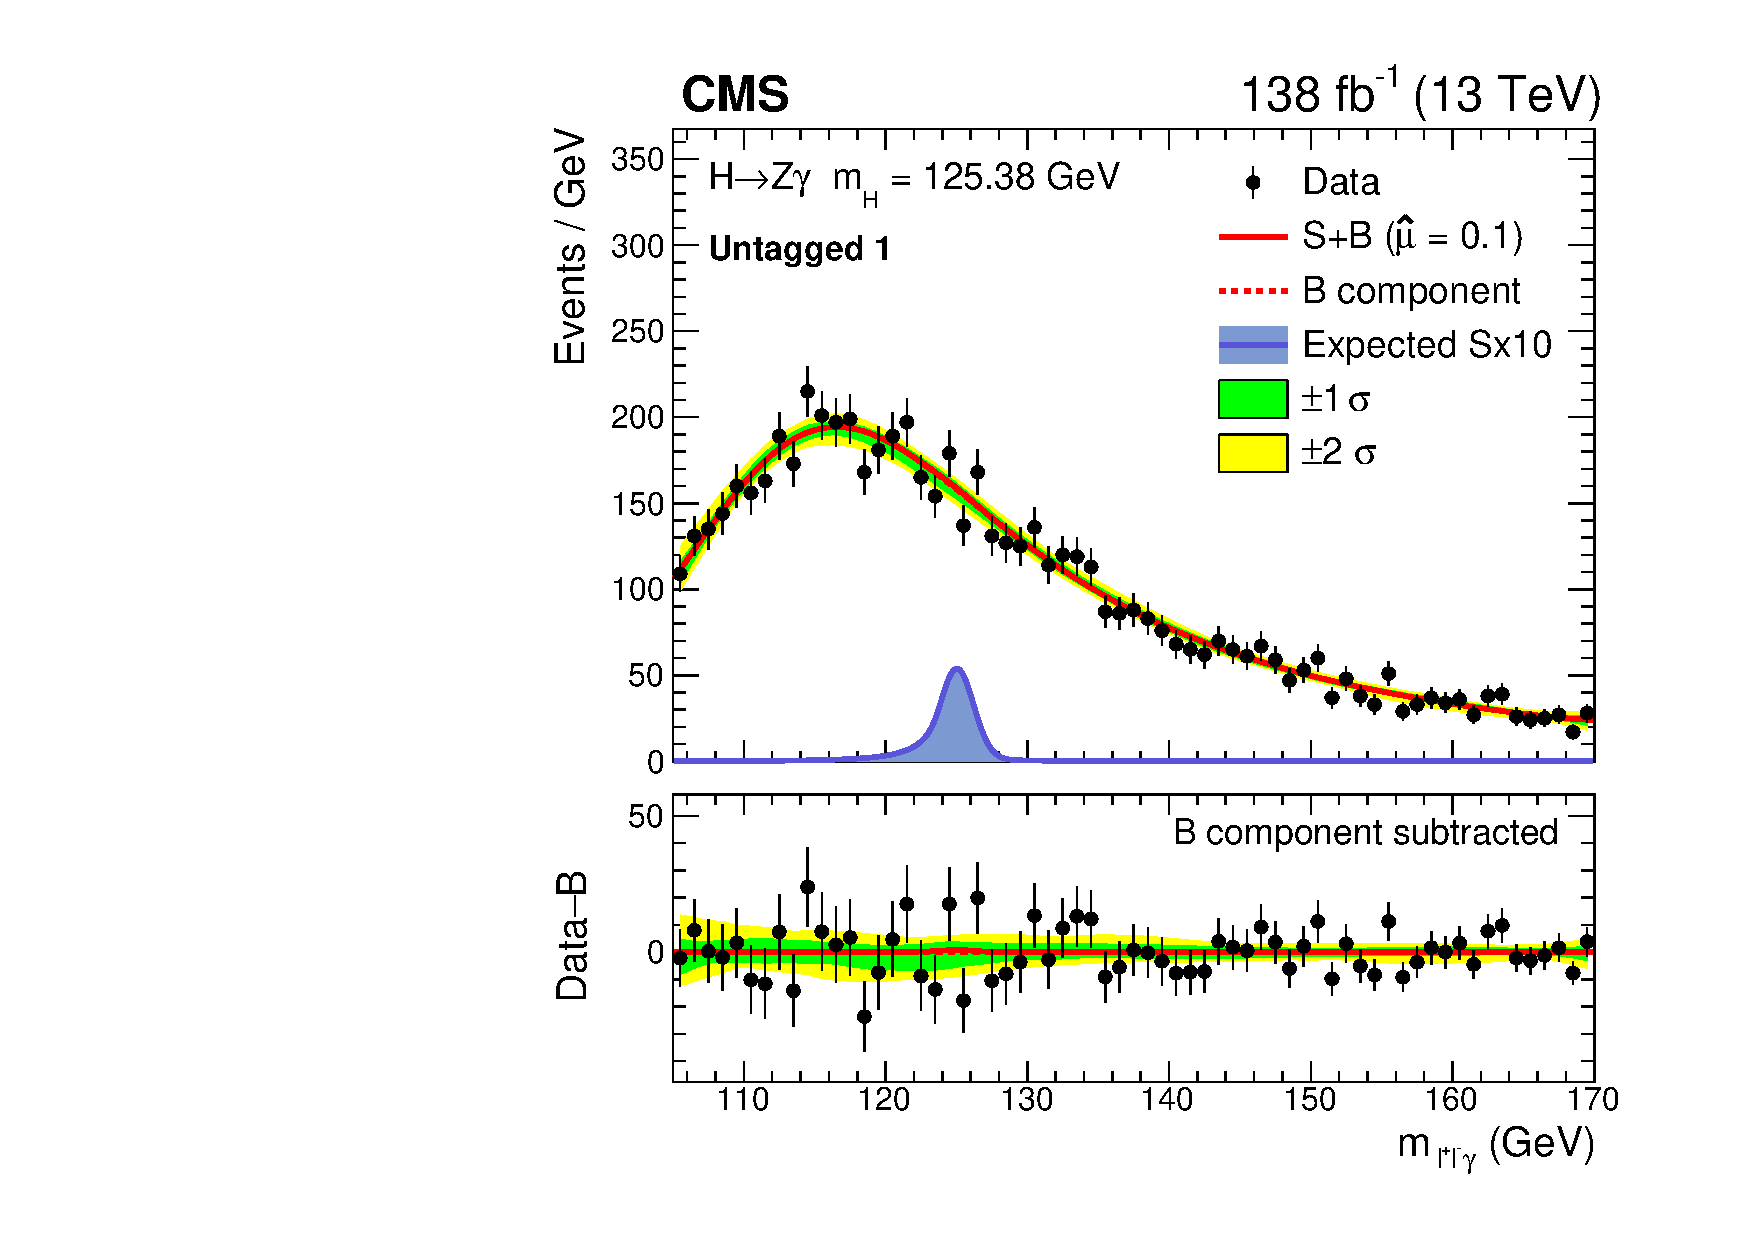
\includegraphics[width=0.45\textwidth]{fig/results/Figure_006-a.pdf}
  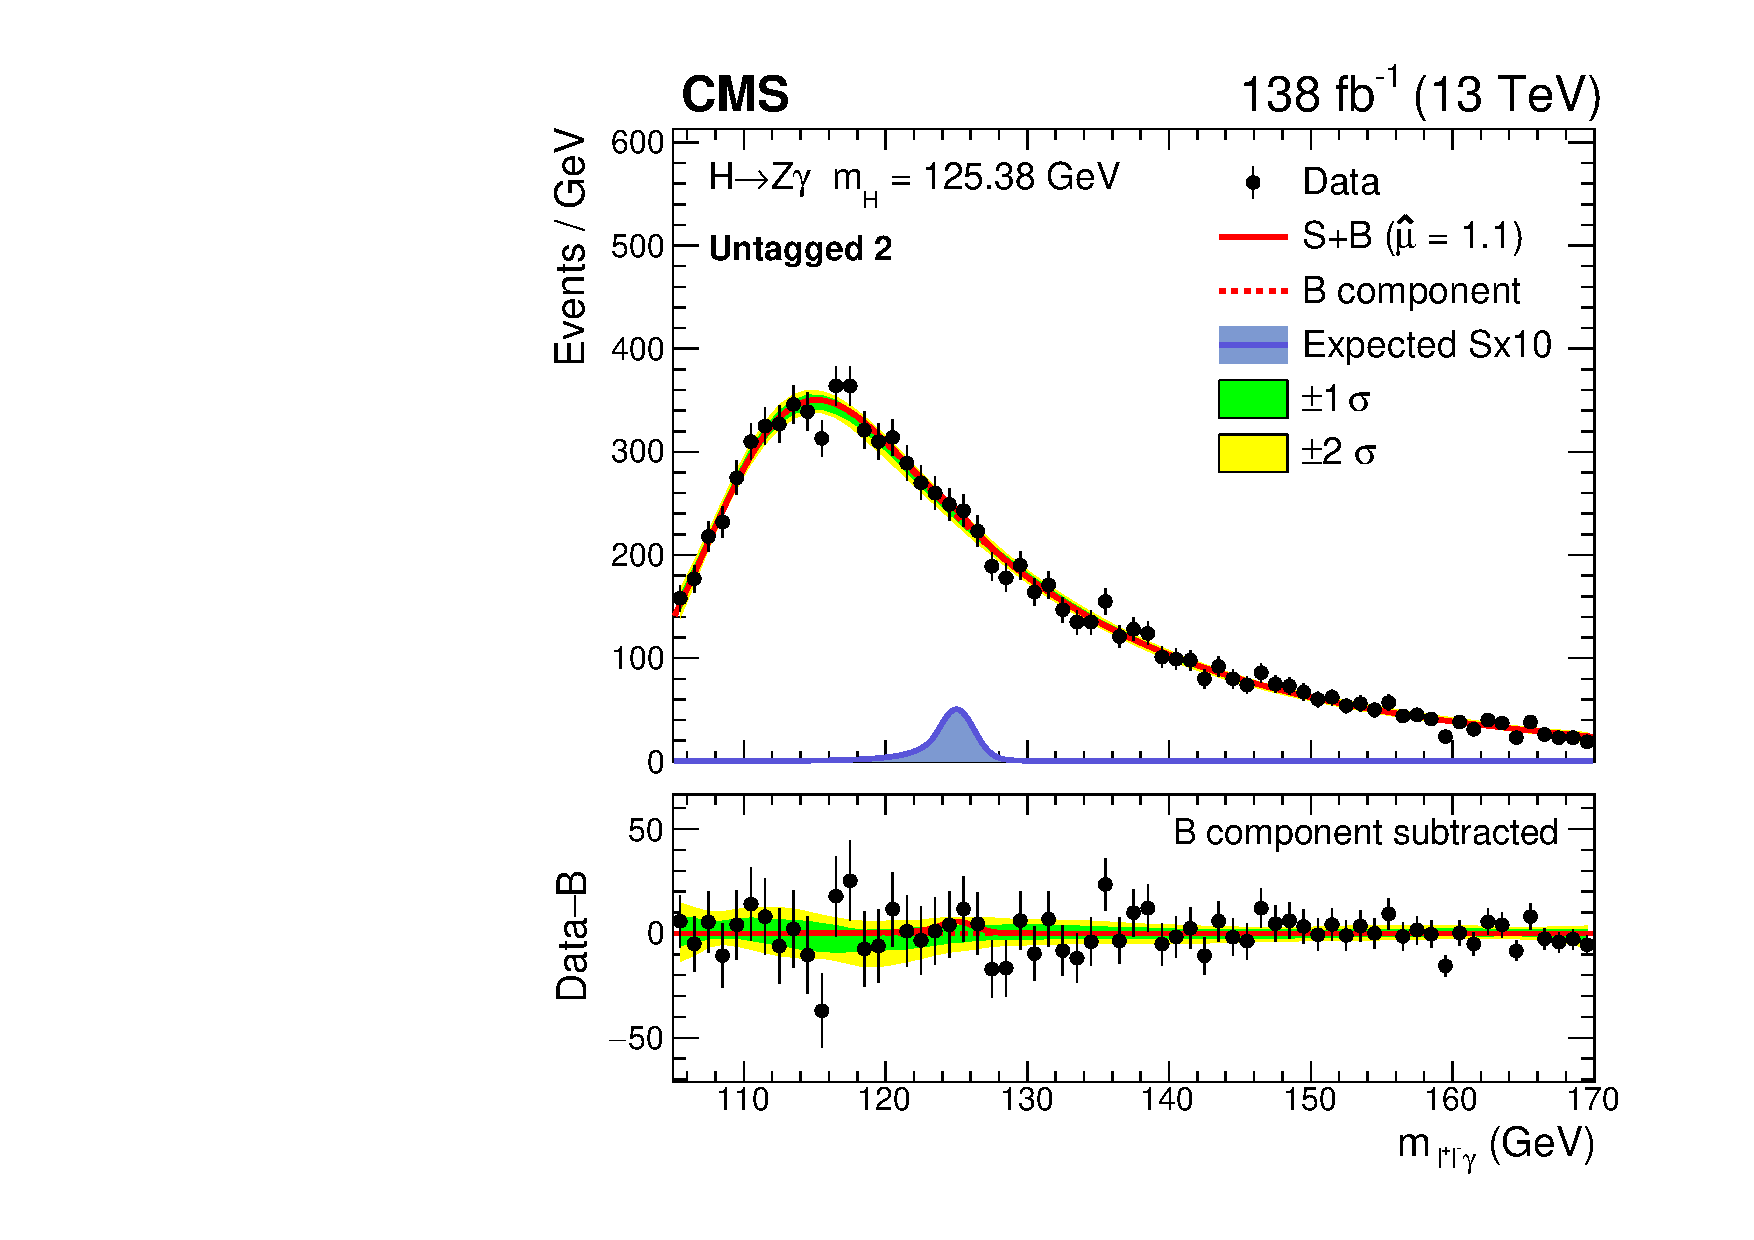
\includegraphics[width=0.45\textwidth]{fig/results/Figure_006-b.pdf}\\
  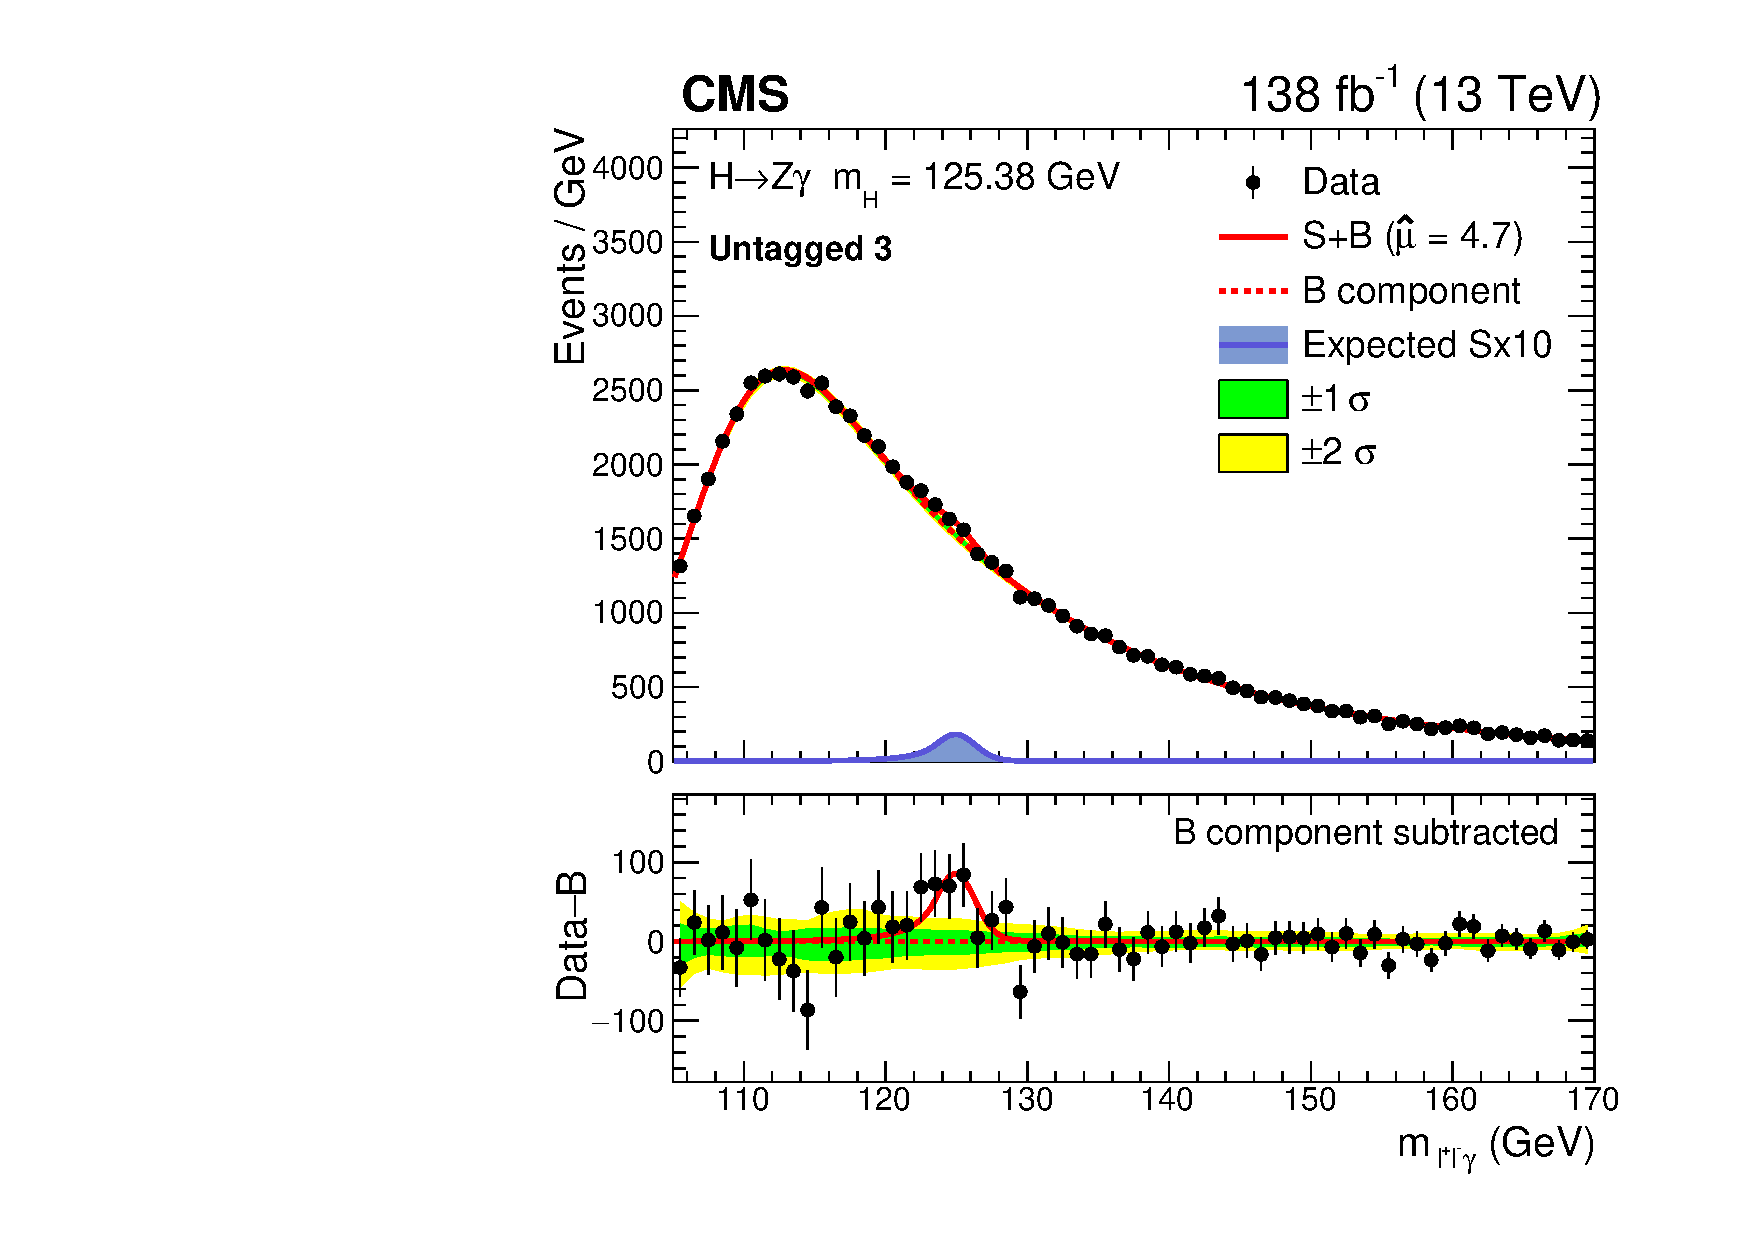
\includegraphics[width=0.45\textwidth]{fig/results/Figure_006-c.pdf}
  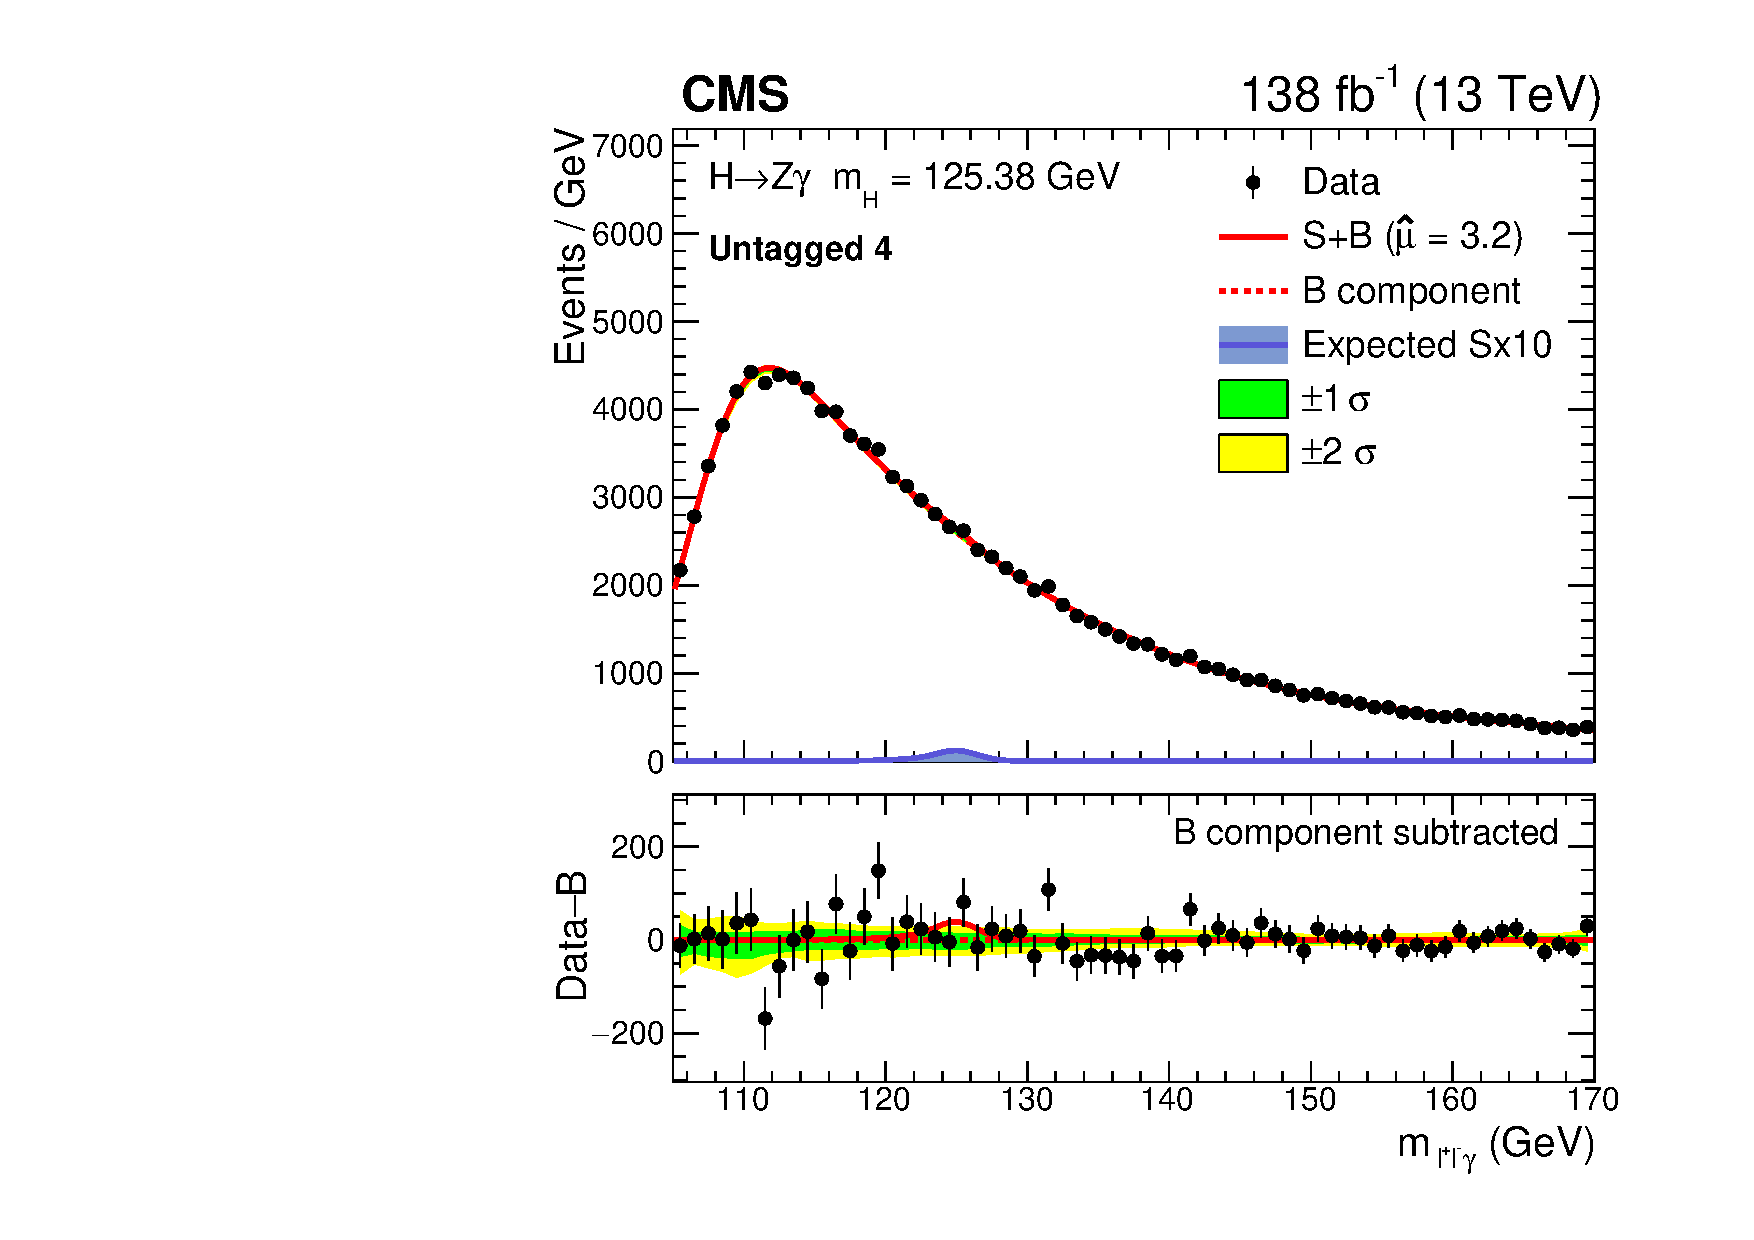
\includegraphics[width=0.45\textwidth]{fig/results/Figure_006-d.pdf}
   \caption{Fits to the $m_{\ell^+\ell^-\gamma}$ data distribution
    in the untagged 1 (upper left), untagged 2 (upper right), untagged 3 (lower left), and
  untagged 4 (lower right) categories.
  In the upper panel, the red solid line shows the result of a signal-plus-background fit to the given category.
  The red dashed line shows the background component of the fit.
  The green and yellow bands represent the $68$ and $95$\% \CL\ uncertainties in the fit.
  Also plotted is the expected SM signal, scaled by a factor of 10.
  In the lower panel, the data minus the background component of the fit is shown. \label{fig:4}}
  \end{figure}

\begin{figure}
\centering
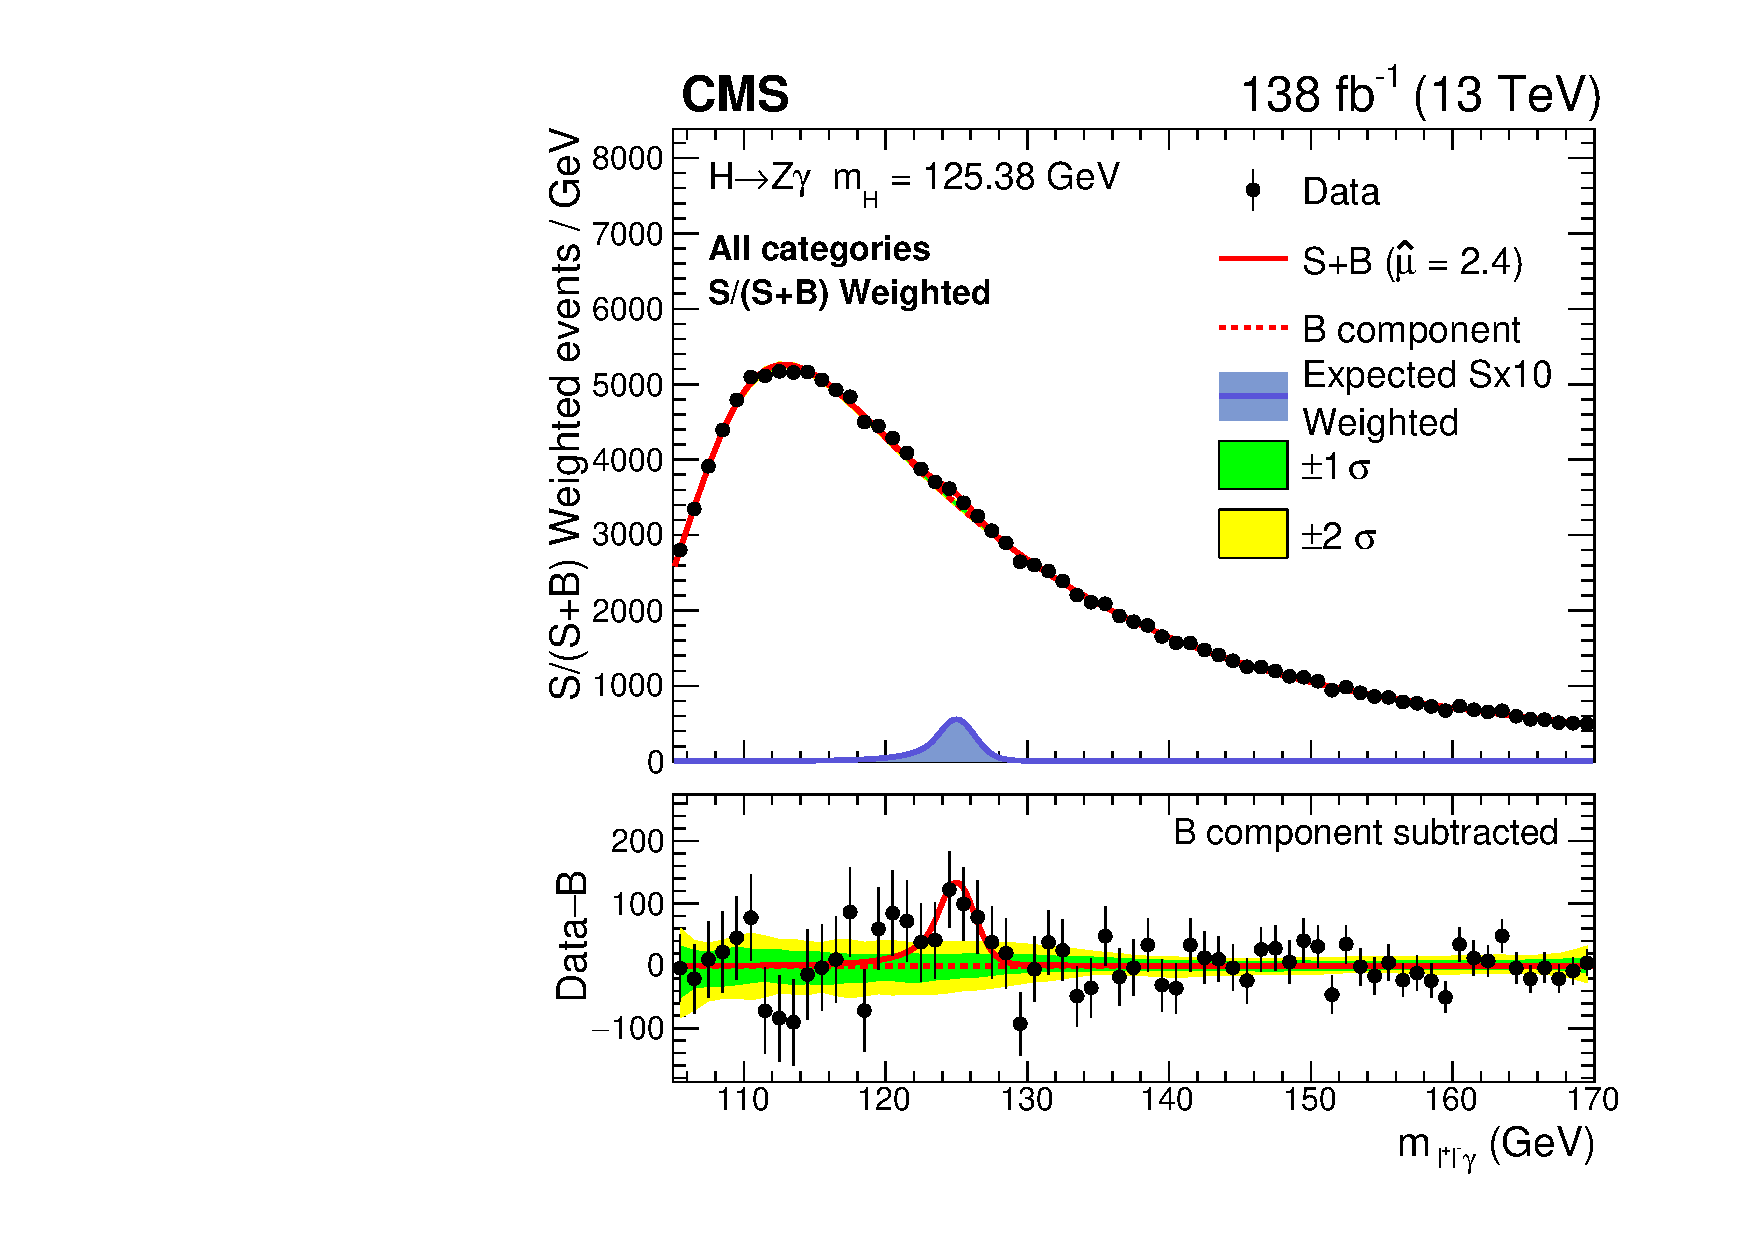
\includegraphics[width=0.5\textwidth]{fig/results/Figure_012.pdf}
 \caption{Sum over all categories of the data points and signal-plus-background model after the simultaneous fit to each $m_{\ell^+\ell^-\gamma}$ distribution. 
 The contribution from each category is weighted by $S/(S+B)$, as defined in the text. 
 In the upper panel, the red solid line shows the signal-plus-background fit. The red dashed line shows the background component of the fit. The green and yellow bands represent the $68$ and $95$\% CL uncertainties in the fit. Also plotted is the expected SM signal weighted by $S/(S+B)$ and scaled by a factor of 10. In the lower panel, the data minus the background component of the fit is shown.
   }
\label{fig:SignalBackground}
\end{figure}

The best fit value of the signal strength is $\signalstrengthExpanded$ at $m_\PH=\mH$\GeV.
The corresponding measured value of $\sigma(\Pp\Pp\to\PH)\mathcal{B}(\PH\to\PZ\gamma)$ is $\brExpanded$\,pb. This measurement is consistent with the SM prediction of $0.09 \pm 0.01$\,pb at the \compatibility\, standard deviation level.
Figure~\ref{fig:lim-combo125} shows the signal strengths obtained for each category separately, corresponding to the fit results shown in Figs.~\ref{fig:3}~and~\ref{fig:4}, as well as from simultaneous fits to the dijet categories, the untagged categories, and all categories combined. 
Among the eight categories, dijet 1 is the most sensitive.
A category compatibility $\textit{p}$-value, under the hypothesis of a common signal strength in all categories, is calculated from the likelihood ratio between the 
nominal combined fit, in which all categories have the same signal strength parameter, 
and a separate fit, in which each category has its own signal strength parameter. 
This $\textit{p}$-value is found to be \channelcompatp, corresponding to \channelcompatsigma\, standard deviations, and is driven by the dijet 3 category, which has a signal strength of $\hat{\mu}=\signalstrengthdijetthree$. 
The observed (expected) local significance is \obssig\,(\expsig) standard deviations. 
Upper limits on $\mu$ are calculated at 1\GeV intervals 
in the mass range of $120 < m_{\ell^+\ell^-\gamma} < 130\GeV$ and at $m_\PH=\mH\GeV$, as shown in Fig.~\ref{fig:lim}.
The observed (expected) limit at 95\% CL relative to the SM expectation for $m_\PH=\mH\GeV$ is $\obslimit$ ($\explimit$). 

\begin{figure}
  \centering
  %  \includegraphics[width=0.75\textwidth]{Figure_010.pdf}
   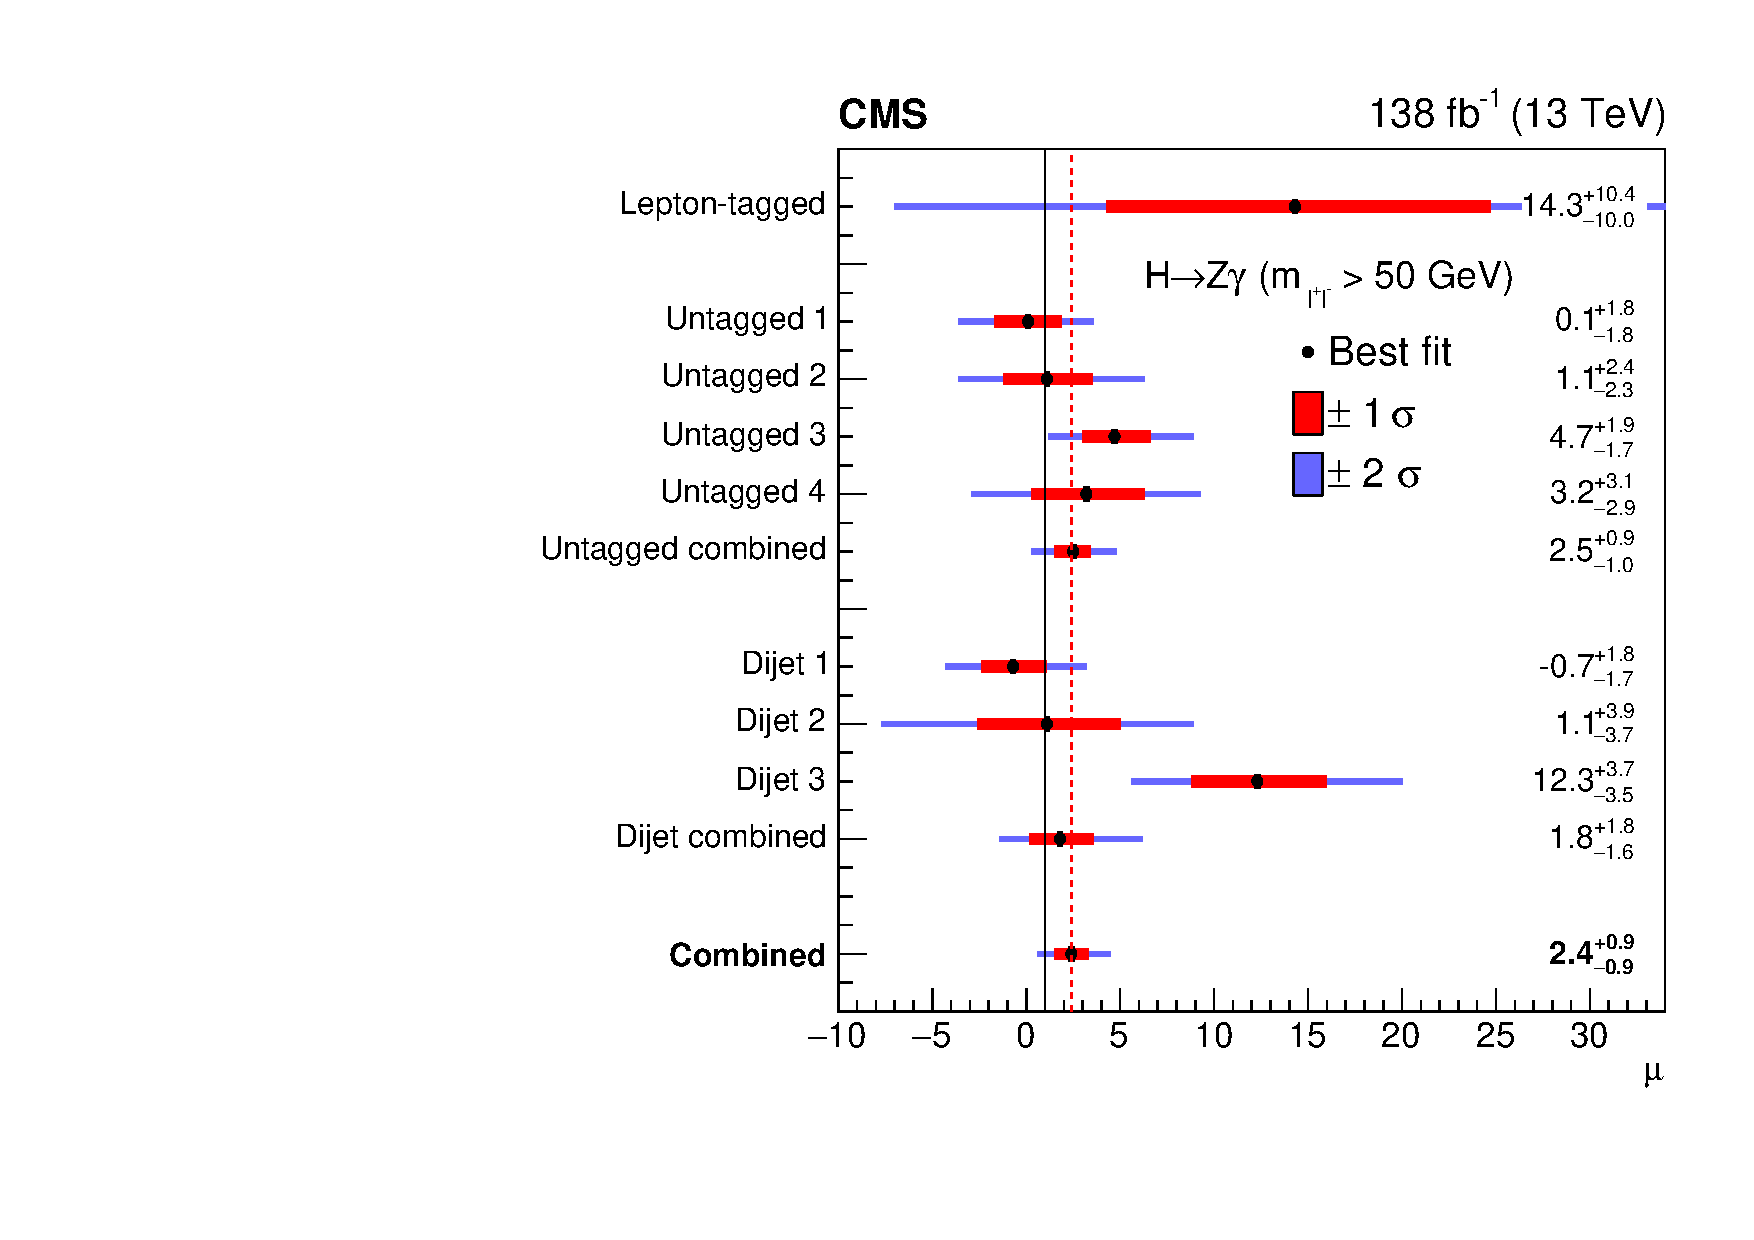
\includegraphics[width=0.7\textwidth]{fig/results/Figure_011.pdf}
    \caption{
Observed signal strength ($\mu$) for a SM Higgs boson with $m_\PH=\mH\GeV$. 
The labels ``untagged combined," ``dijet combined," and ``combined" represent the results obtained from simultaneous fits of the untagged categories, dijet categories, and full set of categories, respectively. 
%Fits perform simultaneously for the combined categories, where the untagged, dijet and all categories are considered. 
The black solid line shows $\mu=1$, and the red dashed line shows the best fit value $\hat{\mu}=\,$\signalstrength ~of all categories combined.
    \label{fig:lim-combo125}}
\end{figure}

\begin{figure}
  \centering
  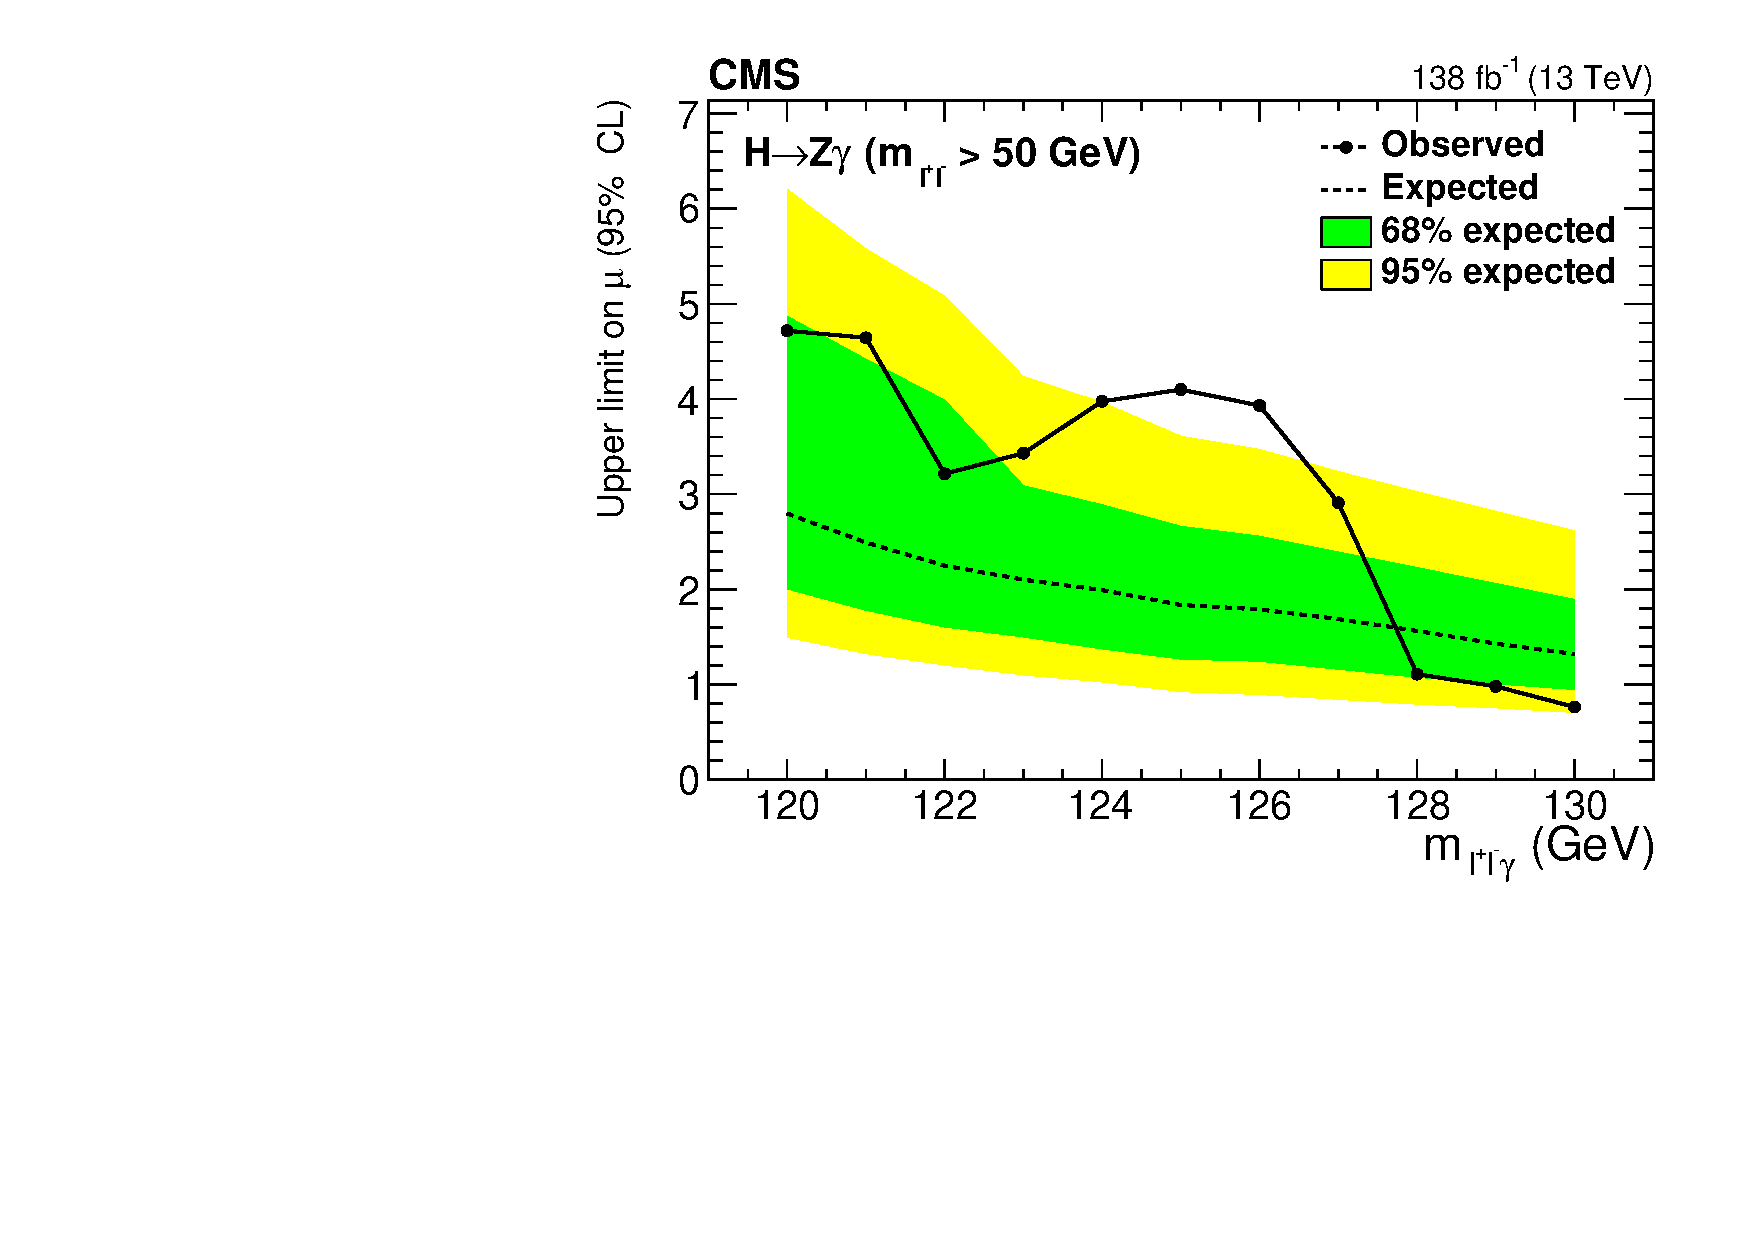
\includegraphics[width=0.7\textwidth]{fig/results/Figure_009.pdf}
    \caption{
	    Upper limit ($95$\%~\CL) on the signal strength ($\mu$) relative to the SM prediction, as a function of the assumed value of the Higgs boson mass used in the fit.
    \label{fig:lim}}
\end{figure}

\section{Ratio Measurement}
The ratio $\mathcal{B}(H\rightarrow\PZ\gamma)/\mathcal{B}(H\rightarrow\gamma\gamma)$ is theoretically interesting, as it is 
potentially sensitive to BSM physics, as described in Chapter~\ref{sec:intro}.
By combining the \hzg{} analysis with the existing CMS $\PH\to\gamma\gamma$ analysis of the same data set~\cite{CMS:2021kom}, 
we can obtain a measurement of this ratio and compare it to the SM prediction of $0.69 \pm 0.04$. 

The profile likelihood scans for the parameters of interest in the ratio fit are shown in Figure~\ref{fig:scan_br}. The best fit values of the 
parameters of interest are $\mu_{\gamma\gamma} = 1.121^{+0.095}_{-0.090}$ and 
$\mu_{Z\gamma}/\mu_{\gamma\gamma} = 2.225^{+0.926}_{-0.825}$. 
The value of $\mu_{\gamma\gamma}$ agrees well with the standalone $\PH\to\gamma\gamma$ fit. 
Multiplying through, the value of $\mu_{Z\gamma}$ is 2.49, which 
agrees well with the result of the standalone \hzg{} fit.
The measured value of $\mathcal{B}(\PH\to\PZ\gamma)/\mathcal{B}(\PH\to\gamma\gamma)$ is \brRatio. 
This measurement is consistent with the SM prediction for the ratio at the \brRatioCompat\, standard deviation level. 

\begin{figure}
   \begin{center}
   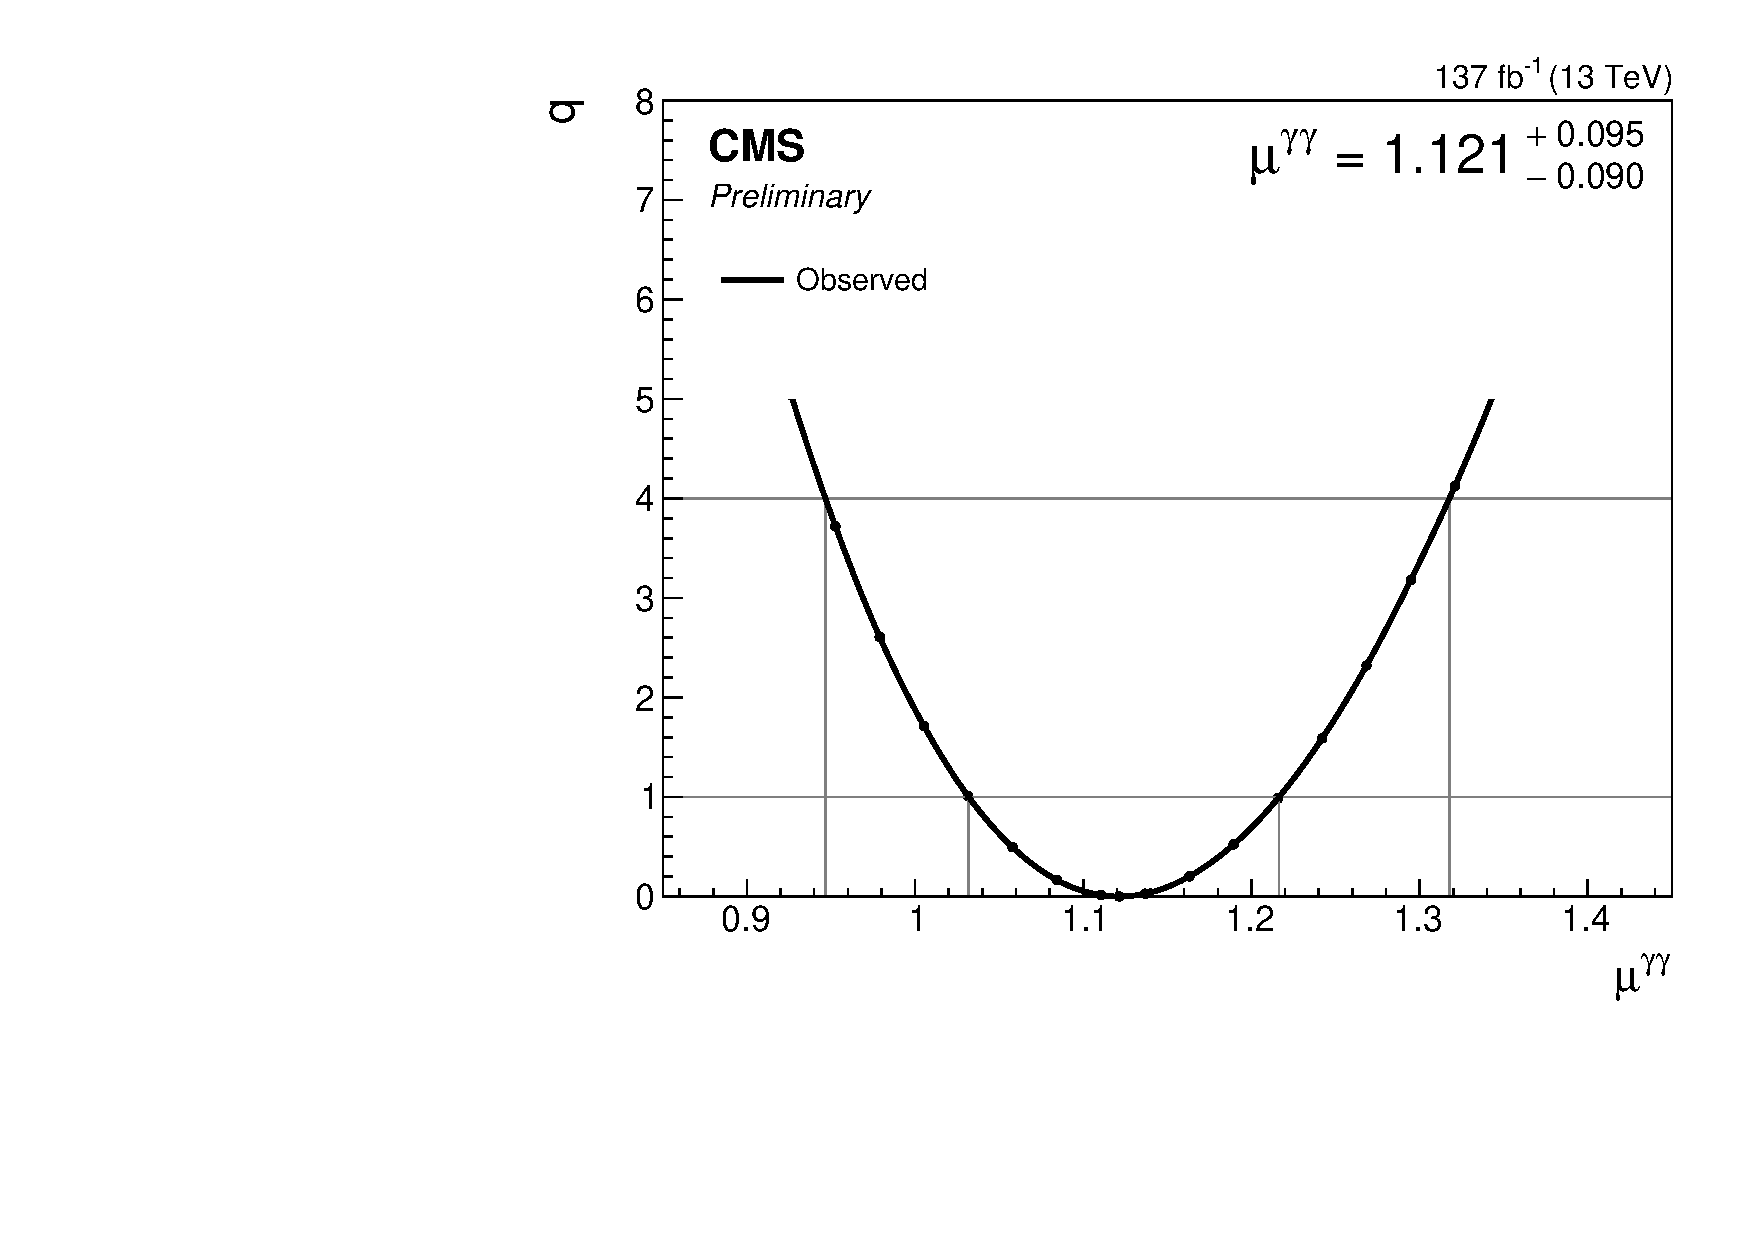
\includegraphics[width=0.45\textwidth]{fig/results/ratio/scan_mu_BR_gamgam.pdf}
   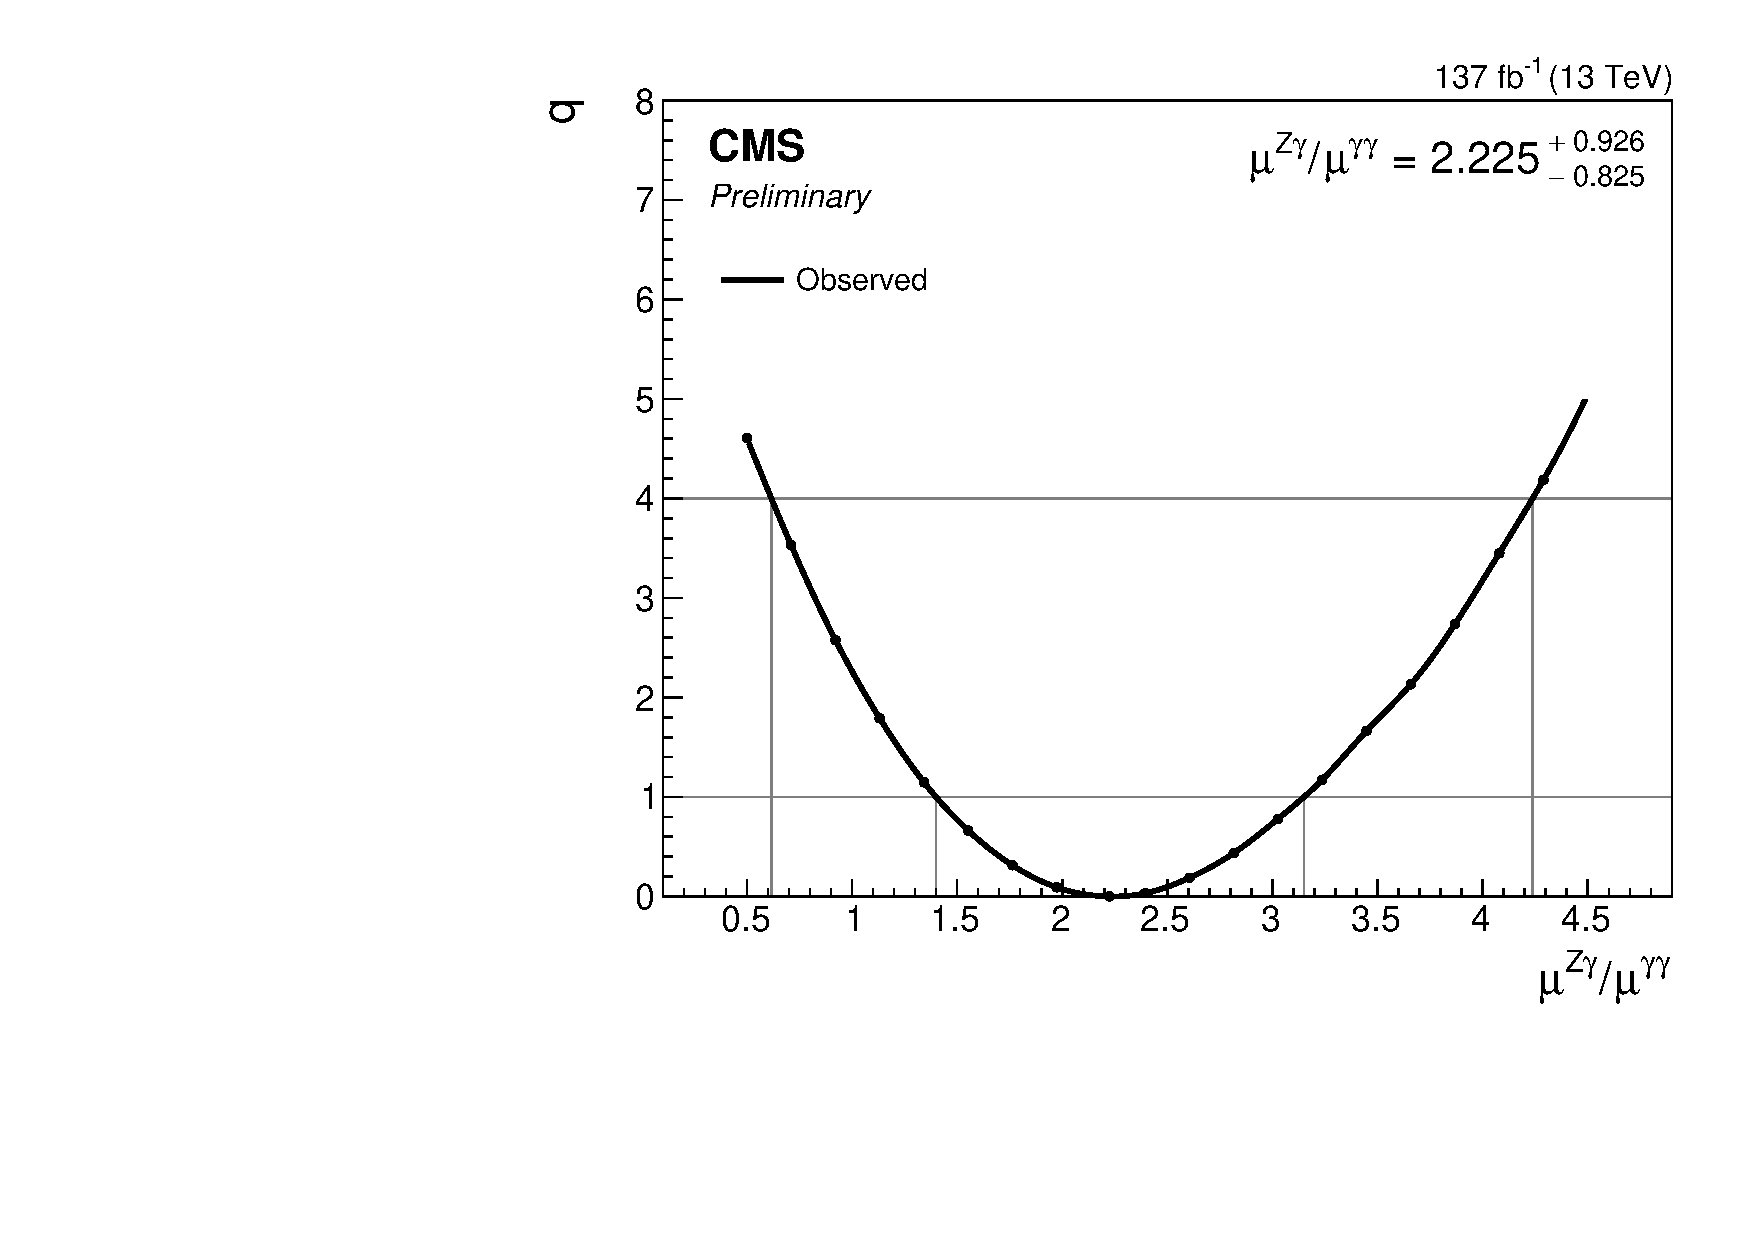
\includegraphics[width=0.45\textwidth]{fig/results/ratio/scan_mu_BR_Zgam_r_BR_gamgam.pdf}\\
   \caption{Profile likelihood scans of $\mu_{\gamma\gamma}$ and $\mu_{\PZ\gamma}/\mu_{\gamma\gamma}$ for $m_H=125.38\GeV$.}
   \label{fig:scan_br}
   \end{center}    
\end{figure}
